\begin{frame}
    \frametitle{\problemtitle}
    \begin{block}{Problem}
    	Given is an undirected graph $G$ of $n$ vertices with binary vertex labels.
    	\begin{itemize}
			\item Find the length of a shortest binary sequence that cannot be obtained by walking in the graph.
			\item If such binary sequence does not exist, print ``\texttt{infinity}''.
    	\end{itemize}
    \end{block}
    \pause
    \begin{block}{When is the answer infinite?}
    	\begin{itemize}
			\item If $G$ is a forest, the answer is finite.
			\item Assume $G$ is a cycle. If the vertex labels follow the pattern ``\texttt{0011001100\dots}'', the answer is infinite.
    	\end{itemize}
	\end{block}
\end{frame}

\begin{frame}{\problemtitle}
    \begin{block}{When is the answer infinite?}
    	\begin{itemize}
			\item If $G$ is a forest, the answer is finite.
			\item Assume $G$ is a cycle. If the vertex labels follow the pattern ``\texttt{0011001100\dots}'', the answer is infinite.
    	\end{itemize}
	\end{block}
	\begin{figure}
		\centering
		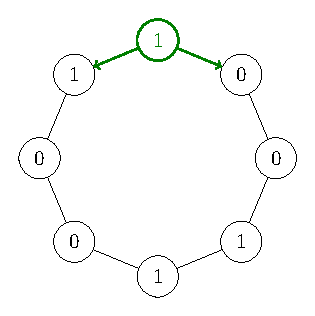
\includegraphics[width=0.3\textwidth]{sol_fig_inf_cycle.pdf}
		\caption{Walking any binary sequence: Both ``\texttt{0}'' and ``\texttt{1}'' can be appended to the sequence.}
	\end{figure}
\end{frame}


\begin{frame}{\problemtitle}
	\begin{block}{When is the answer infinite?}
    	\begin{itemize}
			\item If $G$ is a forest, the answer is finite.
			\item Assume $G$ is a cycle. If the vertex labels follow the pattern ``\texttt{0011001100\dots}'', the answer is infinite.
			\item Similarly, if $G$ contains a closed walk whose labels follow this pattern, the answer is infinite.
			\item Let $G$ contain no closed walk with this pattern. Then there exists a long enough binary sequence that follows this pattern and is not walkable. The answer is thus finite.
		\end{itemize}
    \end{block}
\end{frame}

\begin{frame}
	\frametitle{\problemtitle}
	\begin{block}{Solution}
		\begin{itemize}
			\item Check if the answer is infinite.
			\item If not, consider the longest walks of the following four patterns:\\
			``\texttt{0011001100\dots}'', ``\texttt{'0110011001\dots}'', ``\texttt{1100110011\dots}'' and ``\texttt{1001100110\dots}''.
			\pause
			\item Let the shortest of these walks have length $k$. \textbf{Then the answer is $k+1$}.
			\item Proof sketch: the goal is to prove that any pattern of length $\leq k$ can be walked.
			Any pattern can be "folded" into the form ``\texttt{\dots 00110011 \dots}'', and overlayed on one of the longest walks above.
		\end{itemize}
		Use DP to find for each vertex the longest walk of the four patterns above.
		Runtime: $\mathcal{O}(n)$.
	\end{block}
    \solvestats
\end{frame}
